\documentclass[journal]{IEEEtran}
\usepackage{blindtext}
\usepackage{graphicx}
\usepackage{subfig}
\usepackage[utf8]{inputenc}
\usepackage[brazilian]{babel}
\usepackage{lipsum}
\usepackage{setspace}

\hyphenation{op-tical net-works semi-conduc-tor}

\begin{document}
\onehalfspacing

\title{Representador de Forma de Onda PCM (\textit{Pulse Code Modulation}) - \textit{Delay Modulation}}
\author{Arivanilton dos Santos Araujo Júnior, Rodolfo Bolconte Donato e Ronycley Gonçalves Agra\\

Instituto Federal de Educação, Ciência e Tecnologia da Paraíba\\Campus Campina Grande\\
E-mail: arivanilton.junior@academico.ifpb.edu.br e rodolfobolconte@ieee.org
}


\maketitle


\begin{abstract}
XXXXXXXXXXXXXXXXXXXXXXXXXXXX
\end{abstract}

\begin{IEEEkeywords}
\textit{PCM, Delay Modulation.}
\end{IEEEkeywords}



\section{Definindo a Modulação por Código de Pulso}

Uma grande parte dos sinais de informações que são processados em uma rede de telecomunicações são sinais analógicos, tal como por exemplo o sinal produzido pelo microfone do aparelho telefônico. Para realizar o processamento digital destes sinais, é necessário convertê-los para um formato digital.

A técnica mais conhecida e utilizada para realizar a conversão de um sinal analógico em digital é a modulação por código de pulso, abreviadamente como PCM (\textit{Pulse Code Modulation}). A técnica PCM foi patenteada, em 1939, pelo Sr. Alec. Reeves, quando era engenheiro da \textit{International Telephone \& Telegraph} na França.

A modulação PCM consiste basicamente de três operações separadas: amostragem, quantização e codificação. Na técnica PCM, a informação analógica é inicialmente medida em intervalos regulares de tempo; em seguida, os valores obtidos são aproximados para um dos níveis de referência estabelecidos, e finalmente o valor aproximado é codificado em uma sequência de bits (pulsos).

Existem diversos modos de medir a amplitude das amostras, dando origem a diversas formas de modulação por pulso:

\begin{itemize}
    \item Na Modulação por Amplitude de Pulso (PAM), o sinal de informação é regularmente amostrado em determinados intervalos de tempo, e o valor das amostras é transmitido através de pulsos cuja amplitude é proporcional ao valor do sinal de informação no instante de amostragem;

    \item A amplitude da amostra pode ser também convertida em uma variação da largura de um pulso, resultando na Modulação por Largura de Pulso (PWM);

    \item Pode ser definida também através da variação da posição do pulso no tempo, resultando na Modulação por Posição de Pulso (PPM).

\end{itemize}

Nas modulações PAM, PWM e PPM, a informação contida nos pulsos na forma de amplitude, largura ou posição do pulso é diretamente afetada pelo ruído introduzido no sinal quando este é transmitido, sendo que nestes casos não se pode remover o ruído através da regeneração do sinal.

Na técnica Modulação por Código de Pulso (PCM), a amplitude de cada amostra de sinal é representada por um código de vários bits, sendo cada bit transmitido através de um pulso.  Como cada amostra precisa ser transmitida através de vários pulsos, os mesmos precisam ter sua largura reduzida, aumentando consequentemente a banda passante de canal necessária. No PCM, as deformações na largura e amplitude do pulso passam a ser irrelevantes desde que se possa distinguir claramente a presença e ausência de um pulso. O ruído introduzido durante o transmissão do sinal não é cumulativo, pois ele pode ser removido através de um processo chamado de regeneração, de modo que a qualidade do sinal PCM depende somente do processo de geração do sinal, e não do meio onde o sinal é transmitido. Vale ressaltar que pelo fato de o PCM ser um sinal digital, a informação contida na 'palavra' PCM não sofre atenuação.

\section{Modulação por Código de Pulso - \textit{Delay Modulation}}

XXXXXXXXXXXXXXXXXXXXXXXXXXX


\section{Implementação do \textit{PCM - Delay Modulation}}

O representador de forma de onda PCM foi desenvolvido inteiramente em Python, versão 3, em que foram utilizadas as seguintes bibliotecas: Tkinter (criação de interfaces gráficas), Functools (manipulação de funções), Matplotlib (desenvolvimento de gráficos) e Numpy (cálculos científicos).

Apesar do presente trabalho abordar somente a forma de onda \textit{PCM - Delay Modulation}, no representador foram colocados outros tipos de PCM de acordo com seus grupos:

\begin{itemize}
    \item NRZ: NRZ-L, NRZ-M e NRZ-S;

    \item RZ: Unipolar RZ, Bipolar RZ, RZ-AMI;

    \item Codificação em Fase: Bi \textit{Phase} L, Bi \textit{Phase} M e Bi \textit{Phase} S;

    \item Multi-Nível Binário: Dicode NRZ e Dicode RZ.

\end{itemize}

A interface do representador é simples e de fácil interpretação (Figura XX), no canto superior esquerdo se encontra o menu, com uma caixa de entrada de valores (local para entrar com a sequência de bits a serem convertidos) e embaixo da mesma estão todas as opções de forma de onda PCM do representador, só escolher uma que em seguida - se a sequência de bits for válida - um gráfico com a forma de onda será apresentado do lado direito do menu.

\begin{figure}[!h]
    \centering
    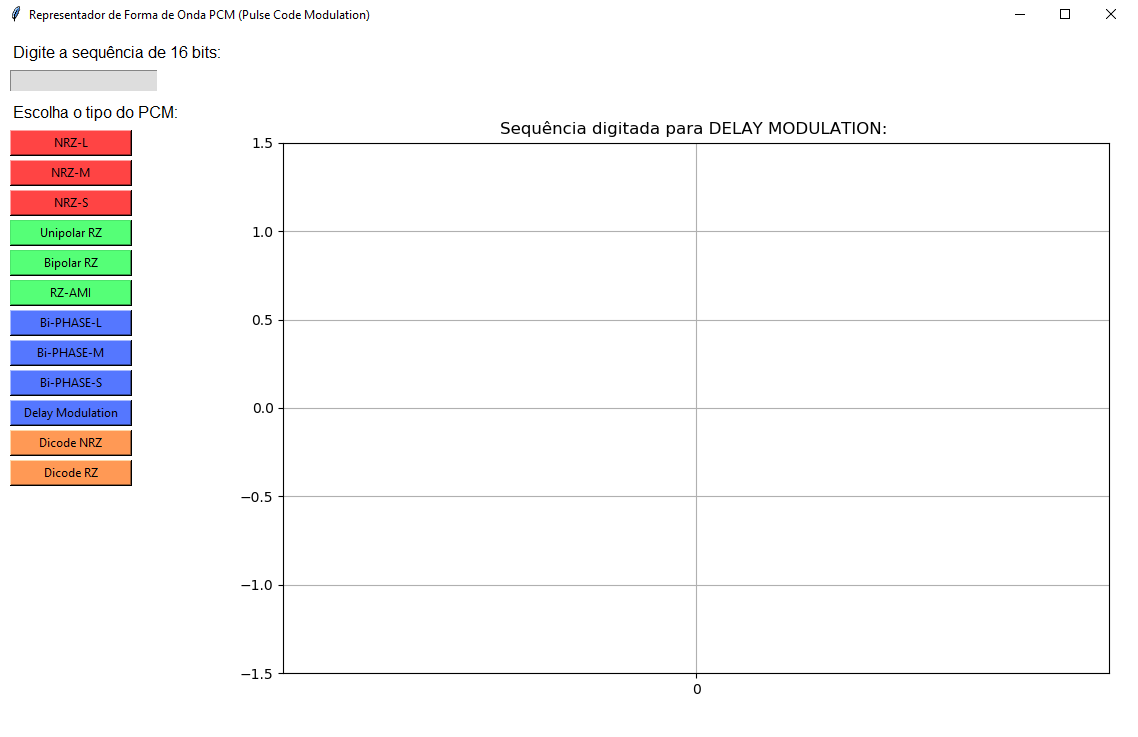
\includegraphics[width=\linewidth]{interface.png}
    \caption{Interface inicial do representador de Forma de Onda PCM desenvolvido.}
\end{figure}

Para a representação gráfica de formas de ondas quadradas, não foi encontrada nenhuma forma destinada somente a este tipo nas bibliotecas gráficas de Python, por este motivo foi aproveitado a função \textit{plot()} da biblioteca Matplotlib que cria um gráfico de marcadores e linhas. Foi utilizado um conceito de taxa de amostragem para cada bit da sequência a ser representada, cada um recebeu 20 amostras (marcadores), sendo esta a quantidade mínima encontrada para uma melhor representação da onda quadrada nas telas dos computadores.

Na Figura XX é possível ver o gráfico criado com a forma de onda PCM - Delay Modulation para a sequência de 16 bits: 1101000110111001.

\begin{figure}[!ht]
    \centering
    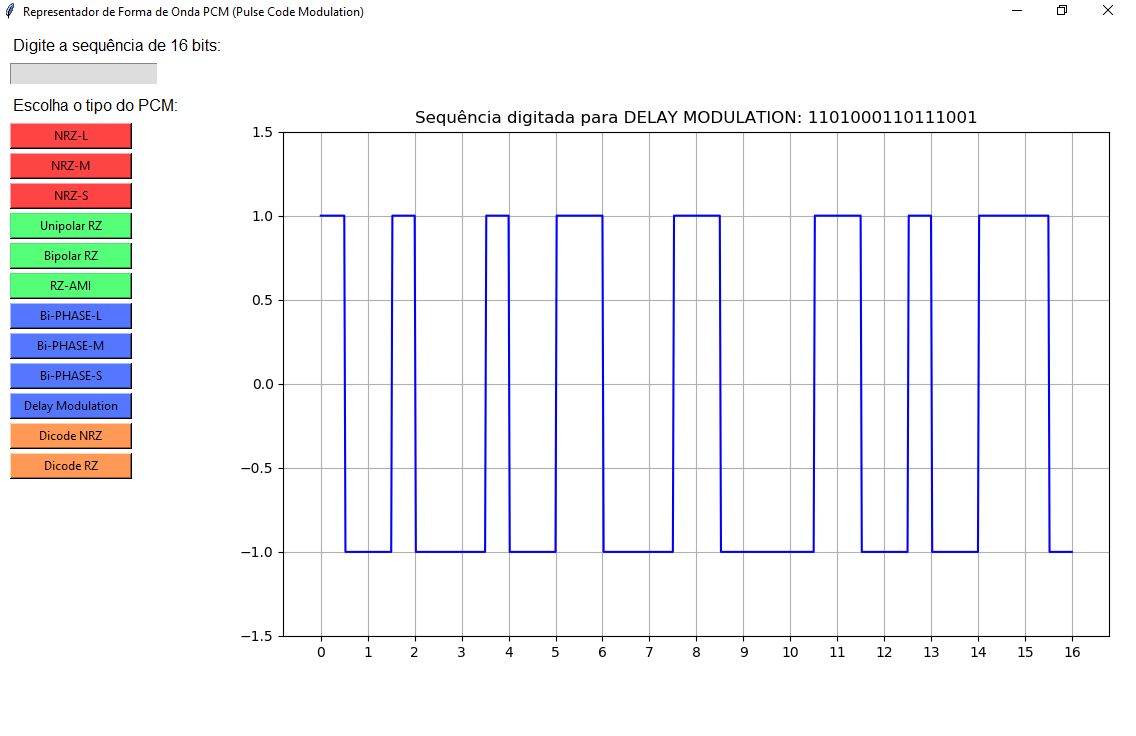
\includegraphics[width=\linewidth]{interface_resultado.png}
    \caption{Forma de Onda PCM Delay Modulation para a Sequência de 16 bits inserida.}
\end{figure}

Todo o código-fonte do representador pode ser encontrado e estudado no GitHub, através do endereço https://github.com/rodolfobolconte/representador\_pcm.


\bibliographystyle{IEEEtran}
\bibliography{referencias}

\end{document}
